% %%%%%%%%%%%%%%%%%%%%%%%%%%%%%%%%%%%%%%%%%%%%%%%%%%%%%%%%%
% | - Active Learning Machine Learning Methodology
% %%%%%%%%%%%%%%%%%%%%%%%%%%%%%%%%%%%%%%%%%%%%%%%%%%%%%%%%%
%   * There will not be much motivation for our general approach from the introduction, so this is a good place to more properly layout our arguments
%
% Points to mention:
%   * Active learning frameworks are a means by which to generate the most valuable training data set, on the fly.
%   * The search space of materials is not a continuous space but a discrete array of individual structures
% __|
%%%%%%%%%%%%%%%%%%%%%%%%%%%%%%%%%%%%%%%%%%%%%%%%%%%%%%%%%%%



% %%%%%%%%%%%%%%%%%%%%%%%%%%%%%%%%%%%%%%%%%%%%%%%%%%%%%%%%%
% | - General intro to AL scheme
%
% __|
% %%%%%%%%%%%%%%%%%%%%%%%%%%%%%%%%%%%%%%%%%%%%%%%%%%%%%%%%%
% | - PARAGRAPH BODY
%
Our approach utilizes an active learning framework and surrogate models,
whereby a regression model is trained to compute enthalpies of formation (\DHf) by iteratively sampling structures from a set of polymorph candidates.
%
Figure~\ref{fig:all_diagram} shows a schematic overview of the AL loop.
%
We first generate the structure candidate space, followed by an iterative search through the space via a continuously retrained surrogate model using Gaussian Processes Regression (GPR),
which is then used to acquire subsequent structures for DFT optimization.
%
No prior DFT training data is required to start the algorithm, eliminating any initial built-in bias in the model and allowing it to quickly respond to new acquisitions.
% __|
%%%%%%%%%%%%%%%%%%%%%%%%%%%%%%%%%%%%%%%%%%%%%%%%%%%%%%%%%%%


% =========================================================
% FIGURE ==================================================
% | - Figure | Active Learning Algorithm ******************
\begin{figure*}[!htb]
\centering
\makebox[\textwidth][c]{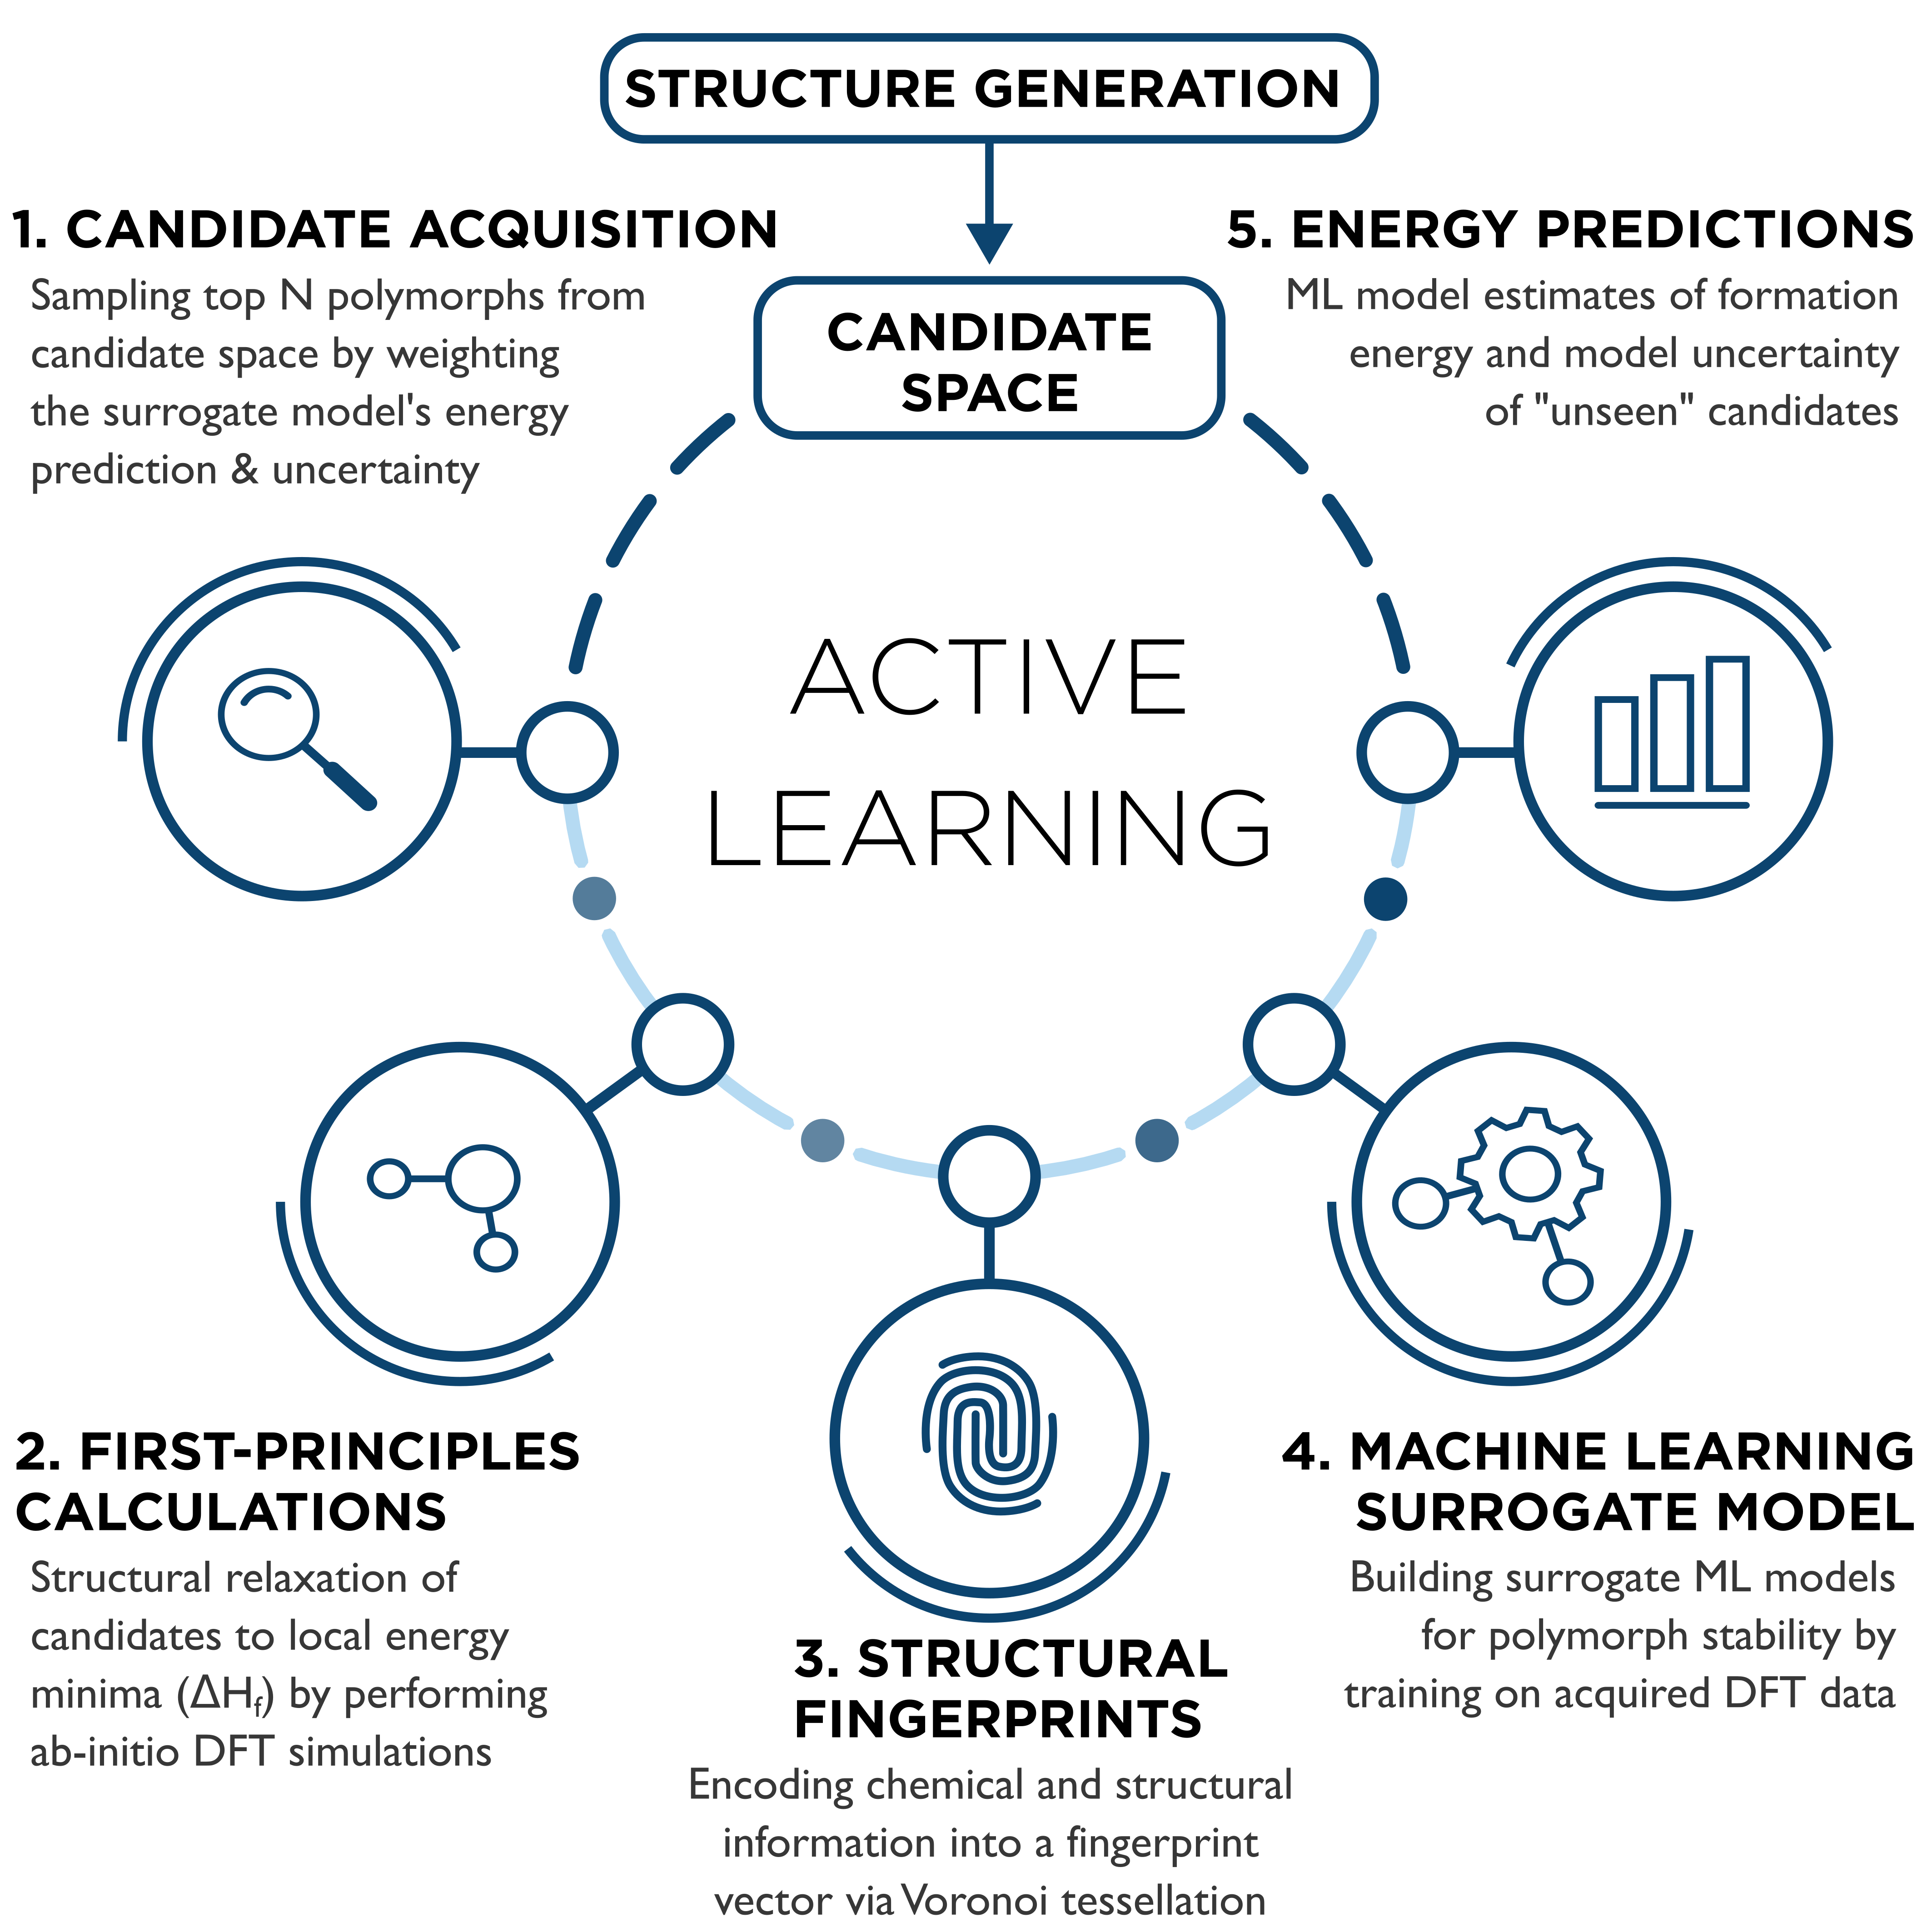
\includegraphics
{02_figures/01_al_process_diagram/Active_learning_diagram__v5__1200dpi.png}}
% {02_figures/01_al_process_diagram/Active_learning_diagram__v5.pdf}}
\caption{\label{fig:all_diagram}
%
AL accelerated polymorph discovery algorithm diagram.
%
Following the generation of the hypothetical crystal structure data set (candidate space),
the AL algorithm proceeds iteratively through:
(1) candidate selection in which a subset of structures in the candidate space are selected based on an acquisition function (in lieu of training data, the initial candidates are randomly sampled),
(2) structural relaxation into local energy minima (\DHf computed),
(3) structure featurization to produce numerical vector for input into ML model,
(4) Machine learning (ML) model training based on acquired structures and \DHf,
(5) Prediction of candidate space's \DHf distribution via ML model.
%
The algorithm repeats steps (1)-(5) until a suitable stop criteria is reached.
}
\end{figure*}
% __|
% =========================================================


% %%%%%%%%%%%%%%%%%%%%%%%%%%%%%%%%%%%%%%%%%%%%%%%%%%%%%%%%%
% | - Candidate Space Generation
%
% __|
% %%%%%%%%%%%%%%%%%%%%%%%%%%%%%%%%%%%%%%%%%%%%%%%%%%%%%%%%%
% | - PARAGRAPH BODY
%
%The generation of the candidate space is a critical step in the discovery of novel crystal structures for a given system,
%since the initial candidate pool determines which structures that can ultimately be discovered, it is imperative to construct candidates that are sufficiently diverse, such that they encompass as much of the structural diversity in the PES as possible.
%
The candidate structure datasets for \IrOtwo and \IrOthree were constructed by first obtaining all \ABtwo and \ABthree structures in the Materials Project\cite{Jain2013} and OQMD\cite{Kirklin2015} databases
(in total \num{7160} \ABtwo and \num{31224} \ABthree entries).
%
To reduce the size of the candidate space while maintaining maximum structural diversity, structurally redundant systems were removed via a space group based structural classification scheme developed by Jain \latin{et al.}~\cite{Jain2018}.
%
In short, a material's structural identity is defined by a unique combination of the element-nonspecific stoichiometry (\ABtwo, \ABthree, etc.), space group symmetry, and Wyckoff positions, collectively referred to as a materials structural prototype.
%
% This is my attempt to further clarify the previous sentence
Materials of the same prototype are considered to be structurally equivalent.
%
%For example, the \num{300000} entry dataset of \ABOthree style perovskites in OQMD, which only differ by the choice of elements for A, B, and C, all belong to the same structural prototype, and are thus structurally equivalent. I don't think this is correct. Let's omit.
%
Eliminating these redundant materials results in orders of magnitude reduction of the search space to \num{697} and \num{259} unique prototypes for \ABtwo and \ABthree, respectively.
%
% The orders of magnitude reduction between all structures and unique structures highlights the lack of structural diversity in the OQMD and MP databases.
%This reduction leads to orders of magnitude reduction of the search space, as opposed to full utilization of the OQMD and Materials Project databases.
%
Finally, only structures containing less than \num{75} atoms
(\num{566} \ABtwo and \num{256} \ABthree)
were included to reduce the computational expense of subsequent DFT calculations.
%
We next substituted iridium and oxygen for the A and B sites, and these Ir-O adapted polymorphs were isotropically relaxed to accommodate their atomic radii.
%
Bulk DFT optimizations were performed on these systems,
yielding \num{714} relaxed bulk \IrOx polymorphs
(\num{466} and \num{248} structures for \IrOtwo and \IrOthree, respectively),
after discarding \num{108} non-converged structures.
%
The relatively small size of our candidate space allows us to tractably optimize all structures and allows us to readily benchmark the performance of our algorithm.
%
Full details of the candidate space generation and DFT calculations can be found in the Supporting Information.
%
All structurally unique \IrOx optimized structures (\num{575} in total) can be accessed through the MPcontribs platform.~\cite{upload_MPContribs}
% __|
%%%%%%%%%%%%%%%%%%%%%%%%%%%%%%%%%%%%%%%%%%%%%%%%%%%%%%%%%%%


% %%%%%%%%%%%%%%%%%%%%%%%%%%%%%%%%%%%%%%%%%%%%%%%%%%%%%%%%%
% | - Featurization Strategy
% Short paragraph on Voronoi featurization
% __|
% %%%%%%%%%%%%%%%%%%%%%%%%%%%%%%%%%%%%%%%%%%%%%%%%%%%%%%%%%
% | - PARAGRAPH BODY
%
The active learning algorithm proceeds through a structure featurization scheme based on Voronoi tessellation developed by Ward \latin{et al.} \cite{Ward2017} which produces a \num{271}-length fingerprint vector that is invariant to isotropic lattice changes and insensitive to the precise atomic coordinates.
%
These fingerprints encode both chemical and structural information by constructing attributes from elemental properties which are weighted by the local environment of the structure via the construction of the Wigner-Seitz cell.
\cite{Wigner1933}
%
Since our AL framework focuses on fixed compositions, the dimensionality is reduced to \num{101} non-zero variance features.
%
% TODO Create cross-validation plot
We further reduce the dimensionality to 10 features via principal component analysis (PCA)~\cite{Tipping1999},
which we found to capture 80\% of the variance in the full feature set while also demonstrating an optimal cross-validation mean absolute error (MAE) (see Figure \ref{fig:cv_anal}).
%
% Further dimensionality reduction was achieved via a principle component analysis (PCA) \cite{Tipping1999}, which was used to reduce the remaining \num{101} fingerprints to \num{10}.
%
% \num{10} PCA components demonstrated the optimal cross-validation mean absolute error (MAE), although only capturing 80\% of the fingerprint's variance (see \ref{fig:cv_anal}).
% __|
%%%%%%%%%%%%%%%%%%%%%%%%%%%%%%%%%%%%%%%%%%%%%%%%%%%%%%%%%%%


% %%%%%%%%%%%%%%%%%%%%%%%%%%%%%%%%%%%%%%%%%%%%%%%%%%%%%%%%%
% | - Active Learning Loop
%
% NOTE This paragraph is a bit long, find way to split into 2
% __|
% %%%%%%%%%%%%%%%%%%%%%%%%%%%%%%%%%%%%%%%%%%%%%%%%%%%%%%%%%
% | - PARAGRAPH BODY
%
The active learning algorithm proceeds through iterative generations of ML training, prediction, and acquisition steps that are visualized in Figure~\ref{fig:all_diagram}.
%
To meet our primary goal of identifying the most stable polymorphs within the candidate space,
we construct the AL framework to be
(1) responsive in improving itself by learning from small batches of newly acquired DFT data,
and (2) aware of limitations in its surrogate model by incorporating uncertainty estimates into the acquisition decision criteria.
%
GPR satisfies both requirements,
and we use them here with a Gaussian kernel as implemented in CatLearn.
\cite{hansen2019atomistic,CatLearn_Repo}
%
In the initial generation (generation 0), the model is trained on a set of randomly sampled candidates (unbiased sampling),
and is then used to predict the formation enthalpy (\DHf) of all structures in the candidate space.
%
The predicted energy landscape is then used to choose the next polymorphs to acquire (calculate via DFT) by selecting systems that minimize the GP-LCB (Gaussian process lower confidence bound) acquisition function,
$U = \mu - \kappa \sigma$~\cite{Cox1992}.
%
Here, $\mu$ and $\sigma$ are the predicted \DHf mean and uncertainty, respectively,
and $\kappa$ is a parameter that weights exploitation vs. exploration of the search-space (set to 1).
%
At every generation of the AL loop, $N$ structures that minimize the acquisition function are acquired for DFT optimization and are subsequently added to the training data set, where $N$ is the AL bin size (here set to 5).
%
% TODO N is used into mean number of atoms (FIX)
The value of $N$ determines the degree of parallelization of the routine.
%
% The optimal value of $N$ depends on the computational resources available, as small values can result in slow down the discovery rate of the AL algorithm,
% as every DFT calculation needs to be performed more serially.
%
% TODO: Is this statement true?
% Larger values of $N$ speed up the active-learning algorithm, but leads to a higher number of DFT calculations performed before convergence.
%
In practice the algorithm can proceed until no more stable polymorphs are found, or after an allocated computational budget is exhausted.
% __|
%%%%%%%%%%%%%%%%%%%%%%%%%%%%%%%%%%%%%%%%%%%%%%%%%%%%%%%%%%%


% %%%%%%%%%%%%%%%%%%%%%%%%%%%%%%%%%%%%%%%%%%%%%%%%%%%%%%%%%
% | - Duplicate Structure Removal
%
% __|
% %%%%%%%%%%%%%%%%%%%%%%%%%%%%%%%%%%%%%%%%%%%%%%%%%%%%%%%%%
% | - PARAGRAPH BODY
%
Although initially unique, the structures in the candidate set often relax into one another over the course of the DFT optimization, introducing duplicates in the post-DFT structures.
%
The duplicates are removed during each generation of the AL algorithm
by using the structure similarity quantification method of Su \latin{et al.}~\cite{Su2017}.
%
% The coordination characterization function (CCF) based methodology to quantify the similarity between structures was used to identify and remove duplicate structures.\cite{Su2017}
% __|
%%%%%%%%%%%%%%%%%%%%%%%%%%%%%%%%%%%%%%%%%%%%%%%%%%%%%%%%%%%
